% Document/LinearAlgebra/VectorSpaces/Foundations/Subspaces.tex
% Section: Vector Subspaces

\newpage
\section{Vector Subspaces}

\begin{definition}[Vector Subspace]\label{def:subspace}
    Let $V$ be a $K$-vector space. A subset $U \subseteq V$ is a \textbf{$K$-vector subspace}
    of $V$ (written $U \Subspace[K] V$) if $U$ is itself a $K$-vector space under the
    inherited operations from $V$.
\end{definition}

\begin{remark}[The Subspace Lattice $\Sub{V}$]\label{rem:sub-lattice}
    We write $\Sub{V}$ for the \textbf{set of all $K$-vector subspaces of $V$}, ordered by
    inclusion. It is a \emph{complete lattice}: any family of subspaces has a meet (intersection)
    and a join (sum):
    \[
        \bigwedge_{i \in I} U_i = \BigIntersect[i \in I] U_i, \qquad
        \bigvee_{i \in I} U_i = \SubspaceSum{i \in I}{U_i}.
    \]
    The bottom element is $\{0\}$ and the top element is $V$. This lattice structure
    underlies the theory of flags (Section~\ref{sec:flags}).
\end{remark}

\begin{example}[Subspaces in Low Dimensions]\label{ex:subspaces-low-dim}
    The following are subspaces:
    \begin{enumerate}
        \item Lines through the origin in $\bb{R}^2$
        \item Lines and planes through the origin in $\bb{R}^3$
        \item $K[X]_{\leq n} \Subspace[K] K[X]$ (polynomials of degree at most $n$)
    \end{enumerate}

    \begin{center}
    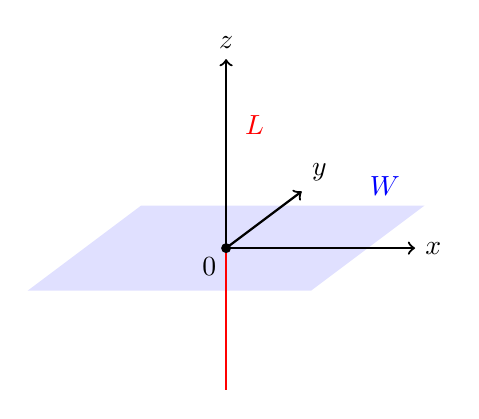
\begin{tikzpicture}[scale=1.2,
        x={(1cm,0cm)},
        y={(0.4cm,0.3cm)},
        z={(0cm,1cm)}]

        % xy-plane (subspace)
        \fill[blue!20, opacity=0.6] (-1.5,-1.5,0) -- (1.5,-1.5,0) -- (1.5,1.5,0) -- (-1.5,1.5,0) -- cycle;
        \node[blue] at (1.2, 1.2, 0.3) {$W$};

        % z-axis (subspace)
        \draw[thick, red] (0,0,-1.5) -- (0,0,1.5);
        \node[red] at (0.3,0,1.3) {$L$};

        % Coordinate axes
        \draw[->, thick] (0,0,0) -- (2,0,0) node[right] {$x$};
        \draw[->, thick] (0,0,0) -- (0,2,0) node[above right] {$y$};
        \draw[->, thick] (0,0,0) -- (0,0,2) node[above] {$z$};

        % Origin
        \fill (0,0,0) circle (1.5pt) node[below left] {$0$};
    \end{tikzpicture}
    \end{center}
\end{example}

\begin{example}[Non-Subspaces]\label{ex:non-subspaces}
    The following are \emph{not} subspaces:
    \begin{enumerate}
        \item A line NOT through the origin in $\bb{R}^2$ (fails: $0 \notin U$)
        \item The first quadrant $\Set{(x, y) \mid x \geq 0, y \geq 0}$ in $\bb{R}^2$
              (fails: not closed under scalar multiplication by $-1$)
        \item The unit circle $\Set{(x,y) \mid x^2 + y^2 = 1}$ in $\bb{R}^2$
              (fails: $0 \notin U$ and not closed under addition)
    \end{enumerate}
\end{example}

\begin{proposition}[Subspace Criterion]\label{prop:subspace-criterion}
    A subset $U \subseteq V$ is a subspace if and only if:
    \begin{enumerate}
        \item $U \neq \emptyset$
        \item $\Forall :{a, b \in K}{\Forall :{u, v \in U}{au + bv \in U}}$
    \end{enumerate}
\end{proposition}

\begin{proof}
    ($\Rightarrow$)
    If $U$ is a subspace, then $U$ is a vector space, so $0 \in U$.
    Closure under linear combinations follows from the vector space axioms.

    ($\Leftarrow$)
    Assume (1) and (2). We verify that $U$ inherits all vector space axioms from $V$:
    \begin{itemize}
        \item \textbf{Closure under addition}: Take $a = b = 1$ in (2).
        \item \textbf{Closure under scalar multiplication}: Take $b = 0$ in (2).
        \item \textbf{Contains zero}: Taking $a = b = 0$ and any $u \in U$ gives $0 \in U$.
        \item \textbf{Additive inverses}: Taking $a = -1$, $b = 0$ gives $-u \in U$.
        \item All other axioms are inherited from $V$.
    \end{itemize}
\end{proof}

\begin{proposition}[Minkowski Characterization of Subspaces]\label{prop:subspace-minkowski}
    For a subset $U \subseteq V$, the following are equivalent:
    \begin{enumerate}
        \item $U$ is a subspace
        \item $U \neq \emptyset$, $U + U = U$, and $KU = U$
        \item $U \neq \emptyset$ and $KU + KU = U$
    \end{enumerate}
    where $KU = \Set{au \mid a \in K, u \in U}$ denotes scalar multiplication of the set.
\end{proposition}

\begin{proof}
    \textbf{(1) $\Rightarrow$ (2)}:
    If $U$ is a subspace, then:
    \begin{itemize}
        \item $U \neq \emptyset$ since $0 \in U$.
        \item $U + U \subseteq U$ by closure under addition. Also $U \subseteq U + U$ since $u = u + 0$ for any $u \in U$.
        \item $KU \subseteq U$ by closure under scalar multiplication. Also $U \subseteq KU$ since $u = 1 \cdot u$ for any $u \in U$.
    \end{itemize}
    Thus $U \neq \emptyset$, $U + U = U$, and $KU = U$.

    \textbf{(2) $\Rightarrow$ (3)}:
    Assume $U \neq \emptyset$, $U + U = U$, and $KU = U$. Then $U \neq \emptyset$ trivially, and $KU + KU = U + U = U$.

    \textbf{(3) $\Rightarrow$ (1)}:
    Assume $U \neq \emptyset$ and $KU + KU = U$. We verify the subspace criterion:
    \begin{itemize}
        \item $0 \in U$: Since $U \neq \emptyset$, pick $u \in U$ and any $\lambda \in K$.
              Then $0 = \lambda u + (-\lambda) u \in KU + KU = U$.
        \item Closure under linear combinations: For any $a, b \in K$ and $u, v \in U$:
              $au + bv \in KU + KU = U$.
    \end{itemize}
\end{proof}

\begin{example}[Trivial Subspaces]\label{ex:trivial-subspaces}
    Every vector space $V$ has two \textbf{trivial subspaces}:
    \begin{itemize}
        \item The zero subspace $\{0\}$
        \item The whole space $V$
    \end{itemize}
    A subspace $U$ with $\{0\} \subsetneq U \subsetneq V$ is called \textbf{proper} or \textbf{nontrivial}.
\end{example}

\begin{definition}[Linear Combination]\label{def:linear-combination}
    Let $V$ be a $K$-vector space and $S \subseteq V$. A \textbf{linear combination} of
    vectors in $S$ is a \textbf{finite} sum
    \[
        \sum_{i \in n} a_i v_i
    \]
    where $n \in \bb{N}$, $a_i \in K$, and $v_i \in S$.

    The empty sum (when $n = 0$) is defined to be $0$.
\end{definition}

\begin{example}[Linear Combinations]\label{ex:linear-combinations}
    Consider the following examples:
    \begin{enumerate}
        \item $3v_1 + 2v_2$ is a linear combination of $\{v_1, v_2\}$
        \item The empty sum $0$ is a linear combination of any set (including $\emptyset$)
        \item In $\bb{R}^3$: $(1, 2, 3) = 1 \cdot e_0 + 2 \cdot e_1 + 3 \cdot e_2$ where $e_i$ are standard vectors
    \end{enumerate}
\end{example}

\begin{remark}[Finiteness is Essential]\label{rem:finite-lincomb}
    Infinite series like $\sum_{i=0}^{\infty} a_i v_i$ are \textbf{not} linear combinations
    in the algebraic sense. Such series require topological structure (limits) to define.

    As a counterexample: in $K^{\bb{N}}$, let $e_i = (0, \ldots, 0, 1, 0, \ldots)$ with $1$ in position $i$.
    Then the constant sequence $(1, 1, 1, \ldots)$ is \textbf{not} a (finite) linear combination
    of the $e_i$'s, even though ``intuitively'' it equals $\sum_{i=0}^{\infty} e_i$.
\end{remark}

\begin{proposition}[Subspace iff Closed Under Linear Combinations]\label{prop:subspace-lincomb}
    $U \Subspace[K] V$ if and only if $U$ is nonempty and closed under all finite linear combinations:
    \[
        \Forall :{F \subseteq U, F \text{ finite}}{\Forall :{(a_v)_{v \in F} \in K^F}{\sum_{v \in F} a_v v \in U}}
    \]
\end{proposition}

\begin{proof}
    This is a reformulation of the subspace criterion. The condition for two vectors
    $au + bv \in U$ implies (by induction) that any finite linear combination is in $U$.
    Conversely, the linear combination condition with $|F| \leq 2$ gives the criterion.
\end{proof}

\begin{proposition}[Linear Combinations of Indicator Functions]%
    \label{prop:lincomb-finite-support}
    Let $I$ be any set and let $(e_i)_{i \in I}$ be the indicator functions in $K^I$.
    Then the set of all linear combinations of the $e_i$'s is precisely $K^{(I)}$.
    In particular, if $I$ is infinite, then there exist elements of $K^I$ that are not
    linear combinations of the $e_i$'s.
\end{proposition}

\begin{proof}
    We show both inclusions.

    ($\subseteq$)
    Let $g$ be a linear combination of the $e_i$'s. Then
    $g = \sum_{j \in n} a_j e_{i_j}$ for some $n \in \bb{N}$, scalars $a_j \in K$,
    and distinct indices $i_0, \ldots, i_{n-1} \in I$. For any $k \in I$:
    \[
        g(k) = \sum_{j \in n} a_j e_{i_j}(k) = \sum_{j \in n} a_j \delta_{i_j k}
        =
        \begin{cases}
            a_j & \text{if } k = i_j \text{ for some } j \in \{0, \ldots, n-1\} \\
            0   & \text{otherwise}
        \end{cases}
    \]
    Hence $\operatorname{supp}(g) \subseteq \{i_0, \ldots, i_{n-1}\}$, which is finite.
    Therefore $g \in K^{(I)}$.

    ($\supseteq$)
    Let $f \in K^{(I)}$. Then $\operatorname{supp}(f) = \{i_0, \ldots, i_{n-1}\}$ is finite.
    Define $g = \sum_{k \in n} f(i_k) \cdot e_{i_k}$. For any $j \in I$:
    \[
        g(j) = \sum_{k \in n} f(i_k) \cdot e_{i_k}(j) = \sum_{k \in n} f(i_k) \cdot \delta_{i_k j}
        =
        \begin{cases}
            f(i_k) & \text{if } j = i_k \text{ for some } k \in \{0, \ldots, n-1\} \\
            0      & \text{otherwise}
        \end{cases}
    \]
    Since $j \notin \operatorname{supp}(f)$ implies $f(j) = 0 = g(j)$, and
    $j = i_k \in \operatorname{supp}(f)$ implies $g(j) = f(i_k) = f(j)$,
    we conclude $f = g$. Hence $f$ is a linear combination of the $e_i$'s.

    For the last claim: if $I$ is infinite, then the constant-$1$ function
    $f(i) = 1$ for all $i \in I$ has $\operatorname{supp}(f) = I$, which is infinite.
    By the first inclusion, $f$ is not a linear combination of the $e_i$'s.
\end{proof}

\begin{proposition}[Intersection of Subspaces]\label{prop:intersection-subspace}
    Let $(U_i)_{i \in I}$ be a family of subspaces of $V$. Then $\BigIntersect[i \in I] U_i$ is a subspace of $V$.
\end{proposition}

\begin{proof}
    Let $U = \BigIntersect[i \in I] U_i$.
    \begin{itemize}
        \item $U \neq \emptyset$: Since $0 \in U_i$ for all $i$, we have $0 \in U$.
        \item \textbf{Closure}: If $u, v \in U$ and $a, b \in K$, then $u, v \in U_i$ for all $i$.
              Since each $U_i$ is a subspace, $au + bv \in U_i$ for all $i$, hence $au + bv \in U$.
    \end{itemize}
\end{proof}

\begin{proposition}[Union of Subspaces]\label{prop:union-subspace}
    Let $U, W \Subspace[K] V$. Then $U \Union W$ is a subspace if and only if $U \subseteq W$ or $W \subseteq U$.
\end{proposition}

\begin{proof}
    ($\Leftarrow$)
    If $U \subseteq W$, then $U \Union W = W$, which is a subspace. Similarly if $W \subseteq U$.

    ($\Rightarrow$)
    Suppose $U \Union W$ is a subspace but $U \not\subseteq W$ and $W \not\subseteq U$.
    Then there exist $u \in U \setminus W$ and $w \in W \setminus U$.
    Since $U \Union W$ is a subspace, $u + w \in U \Union W$.

    \textit{Case 1}: $u + w \in U$. Then $w = (u + w) - u \in U$, contradicting $w \notin U$.

    \textit{Case 2}: $u + w \in W$. Then $u = (u + w) - w \in W$, contradicting $u \notin W$.

    In either case we get a contradiction.
\end{proof}

\begin{proposition}[Minkowski Sum of Subspaces]\label{prop:minkowski-subspace}
    If $U, W \Subspace[K] V$, then $\MinkowskiSum{U}{W} \Subspace[K] V$.
\end{proposition}

\begin{proof}
    We verify the subspace criterion:
    \begin{itemize}
        \item $U + W \neq \emptyset$: Since $0 \in U$ and $0 \in W$, we have $0 = 0 + 0 \in U + W$.
        \item \textbf{Closure}: Let $x = u_1 + w_1$ and $y = u_2 + w_2$ be in $U + W$ (with $u_i \in U$, $w_i \in W$).
              For $a, b \in K$:
              \[
                  ax + by = a(u_1 + w_1) + b(u_2 + w_2) = (au_1 + bu_2) + (aw_1 + bw_2) \in U + W
              \]
              since $au_1 + bu_2 \in U$ and $aw_1 + bw_2 \in W$.
    \end{itemize}
\end{proof}

\begin{definition}[Sum of Subspaces]\label{def:subspace-sum}
    For a family $(U_i)_{i \in I}$ of subspaces of $V$, the \textbf{sum} is
    \[
        \SubspaceSum{i \in I}{U_i} = \Set{\sum_{i \in F} u_i \mid F \subseteq I \text{ finite}, \Forall :{i \in F}{u_i \in U_i}}
    \]
    This is the set of all finite sums with one summand from each subspace in some finite subset of the family.
\end{definition}

\begin{proposition}[Sum of Subspaces is a Subspace]\label{prop:sum-subspace}
    For any family $(U_i)_{i \in I}$ of subspaces, $\SubspaceSum{i \in I}{U_i}$ is a subspace of $V$.
\end{proposition}

\begin{proof}
    Let $S = \SubspaceSum{i \in I}{U_i}$.
    \begin{itemize}
        \item $S \neq \emptyset$: The empty sum (taking $F = \emptyset$) gives $0 \in S$.
        \item \textbf{Closure}: Let $x = \sum_{i \in F} u_i$ and $y = \sum_{j \in G} v_j$ be in $S$.
              For $a, b \in K$:
              \[
                  ax + by = \sum_{i \in F} au_i + \sum_{j \in G} bv_j = \sum_{k \in F \Union G} w_k
              \]
              where $w_k = au_k + bv_k$ if $k \in F \Intersect G$, $w_k = au_k$ if $k \in F \setminus G$,
              and $w_k = bv_k$ if $k \in G \setminus F$. Each $w_k \in U_k$, so $ax + by \in S$.
    \end{itemize}
\end{proof}

\begin{proposition}[Finite Sums Equal Minkowski Sums]\label{prop:finite-minkowski}
    For a finite family $(U_0, \ldots, U_{n-1})$ of subspaces:
    \[
        \SubspaceSum{i \in n}{U_i} = U_0 + U_1 + \cdots + U_{n-1}
    \]
    where the right side is the iterated Minkowski sum.
\end{proposition}

\begin{proof}
    By induction on $n$. For $n = 2$: both sides equal $\Set{u_1 + u_2 \mid u_1 \in U_1, u_2 \in U_2}$.
    The inductive step follows from associativity of the Minkowski sum.
\end{proof}
